%!TEX root = ..//Avali-Arena-Esportivas.tex

\section{INTRODUÇÃO }
\subsection{ Considerações preliminares }
%
\hspace*{1.25 cm}  Arenas esportivas são locais multifuncionais projetados para sediar uma variedade de eventos, incluindo competições esportivas, shows, conferências, futebol e outros tipos de entretenimento.\\ 
%
\hspace*{1.25 cm} No presente trabalho, calculamos tanto o valor da construção e o valor do terreno, com o uso da inferência estatística através do Método dos Mínimos Quadrados - MQO, mostrando que pode ser aplicada na avaliação de estádios de futebol e arenas esportivas, conforme será demonstrado a seguir.\\ 
%
\hspace*{1.25 cm} A amostra adotada neste estudo conta com 16 estádios de futebol distribuídos por todo o Brasil. Esta amostra inicial, com um incremento de mais dados, terá a tendencia de dar maior precisão aos resultados obtidos, permitindo inclusive uma maior opção de variáveis independentes.

\subsection{ Objeto do Estudo de caso }


Este estudo trata da avaliação de um estádio de futebol, para sediar uma variedade de eventos, incluindo competições esportivas, shows, conferências, futebol e outros tipos de entretenimento.
\begin{figure}[H]
	\centering  \small 	\caption{Avaliando - estádio hipotético}
	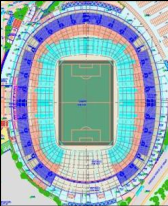
\includegraphics[width=0.347\linewidth]{figura/screenshot001}
	\label{fig:INDICES3}\\{ Fonte:  retirada da internet}
\end{figure}
